\section{Background}

In this section, we discuss the topics that are crucial to understanding the complexities and scope of our research. We begin by exploring the core principles of financial markets with an emphasis on the Forex market. Next, we explore two of the great fields in Machine Learning, Neural Networks and Reinforcement Learning. Lastly, we investigate the intersection of these two branches through an exploration of Deep Reinforcement Learning and how this innovative field can be used for Forex trading.

\subsection{Financial Markets and Trading}

Financial markets play a crucial role in the global economy by facilitating capital flow, ensuring liquidity, and managing risks. They provide a platform for entities to trade assets, hedge financial risks, and fund their operations. Various kinds of markets exist, each with its unique function. Table~\ref{Tables:FinancialMarkets} provides a summary of the primary financial markets and the roles they play in the economy. Although each market serves a distinct purpose, they are interconnected in such a way that actions in one market can influence others, highlighting their significance. The behaviour of these markets is influenced by a range of participants, including investors and major financial institutions whose actions can influence asset prices and market trends. In addition, regulatory bodies play an important role in maintaining the integrity of these markets by enforcing policies that protect investors and contribute to prosperity. Technological advances, such as trading platforms and algorithmic strategies, have made the markets more accessible and sophisticated. However, they also bring challenges such as increased volatility and regulatory uncertainty \cite{brandimarte_introduction_2018}.

\input{Tables/FinancialMarkets}

\subsubsection{Forex Market: Characteristics and Significance}

The Foreign Exchange market, or the Forex market, is a marketplace where currencies are exchanged. It is the world's most liquid market, operating continuously across different time zones due to the involvement of banks and institutions worldwide. Major currency pairs such as EUR/USD and GBP/USD play an important role in this market, as they are the most traded pairs and offer information on geopolitical trends. Forex trading is influenced by many factors such as data availability, political events, interest rates, and the use of leverage. Leverage allows investors to control significant positions with minimal capital, amplifying both potential profits and losses. The unique characteristics of Forex, including its liquidity, diverse participants, and sensitivity to events, make it an attractive topic for advanced financial research and algorithmic strategies. However, given its complex, noisy, and volatile nature, advanced predictive models are required to be able to exploit this type of market, demanding adaptive and intelligence strategies, enhancing the importance of machine learning usage \cite{donnelly_art_2019}.

\subsubsection{Forex Trading: Fundamental Concepts and Operation}

Trading currency pairs involves buying one currency and simultaneously selling another. For instance, when we buy the EUR/USD pair we are essentially purchasing Euros and selling US Dollars based on our prediction that the Euro will strengthen against the US Dollar. In this research, we will be focussing on major currency pairs: EUR/USD, USD/JPY, GBP/USD, AUD/USD, USD/CHF, NZD/USD and USD/CAD. These pairs refer to recognised currencies, mainly European Euro (EUR), US Dollar (USD), Japanese Yen (JPY), Great Britain Pound (GBP), Australian Dollar (AUD), Swiss Franc (CHF) and New Zealand Dollar (NZD). In this way, understanding the value of these pairs offers valuable information on global economic trends, and deciding whether to buy or sell a pair is based on predicting the strength of one currency compared to another \cite{donnelly_art_2019}.

Forex trading occurs in a decentralised market that operates globally. This means that there is no exchange where all transactions take place. Instead, a network of market makers primarily composed of banks (known as the interbank market) and brokers facilitate trades. Interbank transactions involve trades with large volumes, and they are usually dominated by institutions such as multinational corporations and major hedge funds because of their transaction sizes. However, retail traders and small investors can participate in this market through brokers who have access to the interbank network. These brokers serve as intermediaries, facilitating trading for investors by connecting them to the larger currency exchange network. Both market makers and brokers are always ready to buy or sell currencies at quoted prices. The way they operate is by providing two prices publicly: the bid price (the price at which they are willing to buy the pair) and the ask price (the price at which they are willing to sell it). The difference between these two prices, known as the spread, serves as a commission for market makers and brokers. The absence of a central trading venue might suggest a lack of regulation, however, the Forex market is self-regulated by competition among market-makers. This competitive environment ensures that pricing remains fair and spreads are kept tight, thus preserving market integrity and transparency for all participants \cite{donnelly_art_2019}.

To understand the Forex market, it is important to understand how traders interpret market movements. Candlestick charts are a popular approach in this regard as they provide a view of price fluctuations. Each chart is made up of candlesticks, which are structures that represent price movements over a time span that can range from minutes to years. Each individual price movement is known as a tick and occurs when buyers and sellers agree on a price, leading to adjustments in bid and ask prices in the order book. Each candlestick, named for its resemblance to a double-sided candle, provides information on the opening price (O), the highest price (H), the lowest price (L), and the closing price (C) for a specific period of time (see Figure~\ref{Figure:CandlestickChart}). The colour of the candlestick represents the price movement, with lighter shades indicating an increase and darker shades indicating a decrease. This allows traders to gain a fast understanding of the direction of the market just by looking at the chart. Although candlestick charts show price movements, they do not directly show the trading volume (V), which is a measure of the number of ticks or transactions in a given time period, but it is often shown on the chart as an additional indicator of market momentum \cite{rhoads_candlestick_2022}.

\begin{figure}[htb!]
\centering
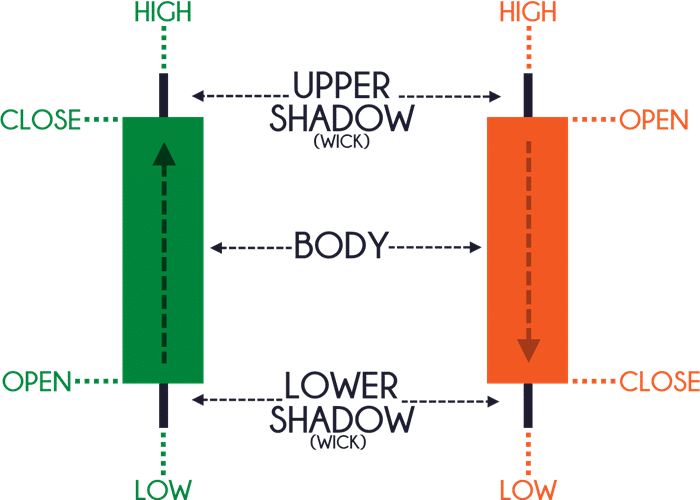
\includegraphics[width=0.4\textwidth]{Images/CandlestickChart.png}
\caption{Candlesticks encoding upward (bullish) and downward (bearish) movements respectively \cite{teo_candlestick_nodate}.}
\label{Figure:CandlestickChart}
\end{figure}

This research will use data containing opening price, highest price, lowest price, closing price and tick volume, or for short, OHLCV data, as it includes all main elements for analysing market behaviour \cite{rhoads_candlestick_2022}. It will also incorporate indicators that interpret this data to provide additional prediction power for the model, as we will see next.

\subsubsection{Financial Analysis: Main Types and Formulas}

Now, we move from representing data in Forex trading to examining it in order to make informed trading decisions, focussing on methods that provide deeper insight into market movement and provide predictive power to the trader. Financial analysis is a complex domain, generally categorised into three main types \cite{lim_handbook_2015}: 

\begin{itemize}
\item \textbf{Fundamental Analysis}: examines economic factors that affect currency prices. This includes analysis of GDP growth, employment rates, interest rates, and monetary policies, which help predict currency trends based on a nation's economic health. However, the qualitative nature of these data poses challenges to computational models that prefer structured numerical input.
\item \textbf{Sentiment Analysis}: seeks to quantify the mood of the market by analysing news, market commentary, and similar qualitative data. It aims to measure how collective emotions impact market trends, although its complexity and need for advanced natural language processing make it less straightforward for model integration.
\item \textbf{Technical Analysis}: involves analysing previous OHLCV data to predict future market movements. It operates on the principle that past market behaviour will repeat itself, and thus identifying past patterns or metrics on current data can predict future movements. It is preferred for its quantitative results, which can be used by complex machine learning models.
\end{itemize}

This research will focus on the use of technical analysis to complement OHLCV data. This type of analysis can be divided into indicators and candlestick patterns. Focussing on indicators, these are metrics created mainly by mathematicians and economists calculated based on historical market data and offer the trader a quantitative approach to understanding market dynamics and predicting future movements. They are generally categorised into four main types \cite{lim_handbook_2015}:

\begin{itemize}
\item \textbf{Trend Indicators}: Used to identify the prevailing direction of the market by filtering out market noise. Refer to Table~\ref{Tables:TrendIndicators} for more details on frequently used indicators.
\item \textbf{Momentum Indicators}: Used to capture the momentum of a given trend, whether it is strong or weak, and if a reversal is expected. Refer to Table~\ref{Tables:MomentumIndicators} for more details on frequently used indicators.
\item \textbf{Volume Indicators}: Used to provide a perspective on the trading volume, providing clues about the strength of a price movement. Refer to Table~\ref{Tables:VolumeIndicators} for more details on frequently used indicators.
\item \textbf{Volatility Indicators}: Used to identify the level of uncertainty or risk associated with the volatility of the price movement. Refer to Table~\ref{Tables:VolatilityIndicators} for more details on frequently used indicators.
\end{itemize}

\input{Tables/TrendIndicators}
\input{Tables/MomentumIndicators}
\input{Tables/VolumeIndicators}
\input{Tables/VolatilityIndicators}

Focussing now on candlestick patterns, unlike indicators which are derived through mathematical calculations of market data, candlestick patterns offer a more visual approach to analysing market movements. These patterns represent price movements in a graphical format that can intuitively signal potential changes in market behaviour \cite{rhoads_candlestick_2022}. Although primarily qualitative, the visual signals provided by candlestick patterns can also be quantified and integrated into machine learning models, allowing for a comprehensive analysis that combines the depth of technical indicators with the intuitive insights of candlestick patterns \cite{jansen_machine_2020}. This dual approach enriches the analytical framework used in predicting future market movements based on historical data.

\subsubsection{Algorithmic and Quantitative Trading}

Financial markets have evolved significantly, increasingly influenced by technology, leading to the predominance of algorithms in trading strategies. Algorithmic trading is a relatively new field of study, using computer programmes to execute trades much faster and in greater volumes than human traders, by leveraging the machines' ability to efficiently analyse large datasets, interpret market conditions, and execute trades based on set criteria. Used in pre-trade analysis, signal generation, and trade execution, algorithmic trading is essential for large institutions and hedge funds to implement complex strategies rapidly and on a large scale. Quantitative trading, driven by quants (quantitative analysts), is a more advanced subfield of algorithmic trading, based on mathematical and statistical models to find trading opportunities. It involves applying these models to market data to identify patterns and correlations, using historical data analysis and machine learning. This data-centric approach demands a strong grasp of finance and mathematics, focussing on systematic strategies over human judgment \cite{chan_quantitative_2021}.

Both algorithmic and quantitative trading have transformed financial markets, enhancing efficiency and introducing new dynamics such as high-frequency trading (HFT). This mix of finance and technology has reshaped trading, highlighting the importance of advanced machine learning models, such as neural networks, for analysing complex market data and reinforcement learning for developing intelligent trading strategies \cite{jansen_machine_2020}.

\subsection{Neural Networks}

In today's world, where we have an abundance of data and easy access to it, the power of machine learning has become a game changer in many fields. At its core, machine learning relies on algorithms to identify patterns in data and to make decisions with minimal human intervention. Tom Mitchell, a leading figure in the field, explains it as \cite{mitchell_machine_1997}:
\begin{quote}
"A computer program is said to learn from experience E with respect to some task T and some performance measure P, if its performance on T, as measured by P, improves with experience E."
\end{quote}
This captures the essence of machine learning: creating models that automatically improve through experience. Neural networks, the topic of this section, are a class of machine learning models that operate within this framework by simulating the complex networks of the human brain.

\subsubsection{Fundamentals and History}

Neural Networks (NN), named for their similarity to the structure of the human brain, are algorithms designed for pattern recognition. In the human brain, a neuron receives signals through structures called dendrites, processes these signals in the nucleus, and passes the resultant processed signal down its axon to the dendrites of adjacent neurons. Similarly, in a neural network, each node represents an artificial neuron that receives input, processes it through a mathematical function, and passes the output to the subsequent layer of nodes. In both cases, the strength and nature of the connections between neurons determine the behaviour of the network \cite{goodfellow_deep_2016}. Refer to Figure~\ref{Figure:HumanNeuronVsArtificialNeuron} for a visual representation of the concepts explained above.

\begin{figure}[htb!]
\centering
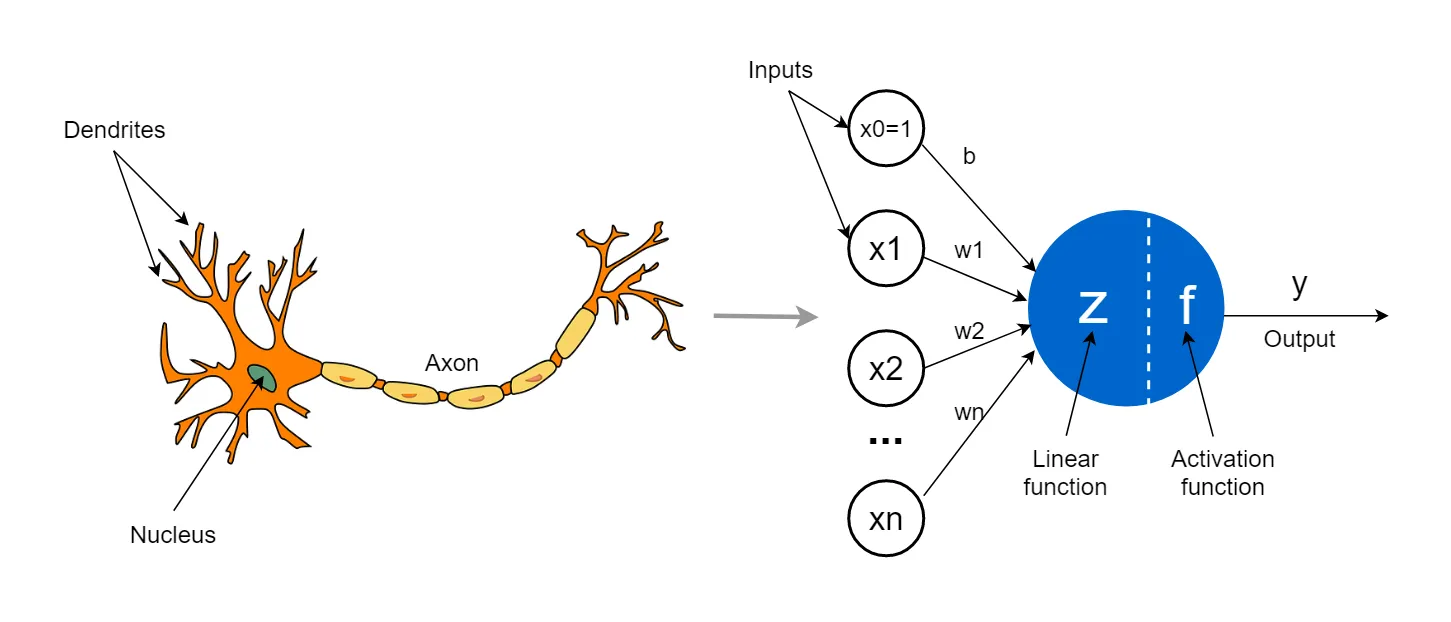
\includegraphics[width=0.7\textwidth]{Images/HumanNeuronVsArtificialNeuron.png}
\caption{Human Neuron compared to an Artificial Neuron \cite{pramoditha_human_nodate}.}
\label{Figure:HumanNeuronVsArtificialNeuron}
\end{figure}

The concept of neural networks dates back to the 1950s with the perceptron, a simple model of a biological neuron developed by Frank Rosenblatt \cite{rosenblatt_perceptron_1958}. The perceptron marked the early stages of NN research, but was limited to linearly separable datasets, leading to some periods of reduced interest in the field, known as "AI winters." However, the 1980s brought a significant breakthrough with the backpropagation algorithm, enabling neural networks to learn patterns in non-linearly separable datasets using complex and multilayered models \cite{rumelhart_learning_1986}.

\subsubsection{Key Concepts and Feed-Forward}

In a neural network, the feed-forward computation within each layer \( l \) is based on the data processed by its predecessor. For the first layer, this input \( x \) is the raw data itself, while for subsequent layers, it is the output of the previous layer \( h^{(l-1)}(x) \). The computation in each layer can be formalised as \cite{goodfellow_deep_2016}:

\begin{equation}
z^{(l)}(x) = W^{(l)} h^{(l-1)}(x) + b^{(l)}
\end{equation}

Here, the weight matrix \( W^{(l)} \in \mathbb{R}^{K_l \times K_{l-1}} \) and the bias vector \( b^{(l)} \in \mathbb{R}^{K_l} \) are required for the computation at layer \( l \), with \( K_l \) representing the number of neurons or units in layer \( l \), and \( K_{l-1} \) indicating the number of neurons in the preceding layer \( l-1 \). In particular, \( W^{(1)} \in \mathbb{R}^{K_1 \times D} \) for the first layer, where \( D \) is the size of the input data. The activation function \( g \) is subsequently applied to the pre-activation \( z^{(l)}(x) \in \mathbb{R}^{K_l} \) to produce the activated output \( h^{(l)}(x) \in \mathbb{R}^{K_l} \) \cite{goodfellow_deep_2016}:

\begin{equation}
h^{(l)}(x) = g(z^{(l)}(x))
\end{equation}

During the design of a neural network, the choice of activation functions is very important. Starting by the hidden layers, we may employ a variety of non-linear activation functions, adding layers of expressiveness to the network and allowing it to learn more complex patterns. Finally, the activation function used in the output layer is determined by the type of task the network is going to perform. This careful selection directly influences the network's ability to accurately and effectively model the dataset \cite{goodfellow_deep_2016}. Refer to Table~\ref{Tables:ActivationFunctions} for a summary of the most common activation functions.

\input{Tables/ActivationFunctions}

\subsubsection{Learning using Backpropagation}

Neural networks learn by iteratively adjusting weights and biases to minimise the error between predicted outputs and actual target values. This learning process is guided by a loss function that quantifies the model's error. The goal is to optimise the network by finding parameters that minimise this loss function. Different problems require different loss functions, such as mean squared error for regression tasks and cross-entropy for classification \cite{goodfellow_deep_2016}. Refer to Table~\ref{Tables:LossFunctions} for a detailed overview of their formulas.

\input{Tables/LossFunctions}

The core algorithm used to train neural networks is known as backpropagation \cite{rumelhart_learning_1986}. It involves calculating the gradients of the loss function relative to the network's weights and biases, which mathematically indicate the steepest increase in the loss function. Refer to Algorithm~\ref{Codes:GradientLossFunction} for a detailed overview of how to calculate these gradients. Then, gradient descent algorithm is used to iteratively update the weights and biases in the opposite direction of the gradients, thus reducing the loss and hopefully increasing the network's accuracy. Its variants, outlined with the respective formulas in Table~\ref{Tables:GradientDescent}, address different data and computational needs. Batch gradient descent uses the entire dataset for updates, ensuring completeness but potentially struggling with large datasets. Stochastic gradient descent updates the parameters per data point, offering speed at the cost of stability. Mini-batch gradient descent strikes a balance, using data subsets for more stable and computationally efficient updates \cite{goodfellow_deep_2016}.

\input{Codes/GradientLossFunction}

In Table~\ref{Tables:GradientDescent}, the learning rate \( \eta \) is an hyperparameter that influences the convergence of gradient descent. An optimal learning rate balances convergence speed and precision, preventing overshooting or slow progress that could get trapped in local minima. Adaptive learning rate techniques by adjusting \( \eta \) during training improve learning efficacy, emphasising the balance between convergence speed and accuracy in neural network training. Some other techniques to improve convergence and its speed involve normalisation and standardisation of the input data \cite{goodfellow_deep_2016}.

\input{Tables/GradientDescent}

\subsubsection{Bias-Variance Trade-off and Model Generalisation}

The generalisation power of a neural network depends on finding a balance between bias and variance. Bias leads to underfitting, where the model overlooks underlying trends due to overly simplistic assumptions, while variance leads to overfitting, where the model interprets noise as a signal due to excessive complexity. Both underfitting and overfitting result in poor performance of the model on new data, a significant issue in Forex trading, where accurate market signal detection is essential. To prevent this, cross-validation is commonly employed to evaluate a model's generalisation power in independent training, validation and testing datasets. Regularisation techniques such as L1 and L2 are also used to moderate the model complexity by adding penalties to the loss function. Furthermore, principal component analysis (PCA) can help to find the right balance between bias and variance by selecting, extracting and generating relevant features to the model. Implementing these strategies increases the change of training a model with more generalisation power, thus allowing it to perform in out-of-sample data \cite{goodfellow_deep_2016}. Although important, these techniques are not the main focus of this research and will not be explored in full detail.

\subsubsection{Universal Approximation Theorem}

The universal approximation theorem, formalised by Kurt Hornik in 1989, states \cite{hornik_multilayer_1989}:

\begin{quote}
"A Neural Network with one hidden layer and a linear output can approximate arbitrarily well any continuous function, given enough hidden units."
\end{quote}

This validates the capacity of neural networks to serve as universal function approximators, which is an important result in the context of creating predictive models for Forex trading because, in theory, they should be able to capture the complex underlying patterns that drive market movements, in conjunction with reinforcement learning, as we will see in the next sections.

\subsection{Reinforcement Learning}

Reinforcement Learning (RL) is a type of machine learning that focusses on an agent's ability to interact with its environment and make decisions. Unlike other types of learning methods, RL emphasises decision-making in potentially complex and uncertain environments. The goal of RL is to maximise rewards by learning from the consequences of actions, through trial and error. This approach has found applications in a range of fields such as robotics and finance, enabling the development of systems that improve their performance over time and adapt to new situations and make a series of decisions to achieve desired outcomes.

\subsubsection{Fundamentals and History}

Reinforcement Learning is a field of study that emerged from the combination of many other fields like psychology, computer science, and control theory, and it was inspired by the way humans and animals learn from their environment. RL involves an agent that makes decisions, receiving rewards or penalties based on its actions, aiming to maximise positive outcomes over time. This process is deeply rooted in the concept of operant conditioning, a type of learning discovered by psychologists like B. Skinner \cite{skinner_operant_1963}, where animal behaviour is shaped by its consequences. 

In the 1960s, Markov Decision Processes (MDPs) were introduced, which are frameworks that model decision making where the outcomes are partly random and partly under the control of the decision maker. This new field was the mathematical backbone of RL, as it allowed the development of algorithms that could learn optimal strategies in complex environments. One of the major breakthroughs in RL was the introduction of Q-Learning in the late 1980s, an algorithm capable of learning the value of actions in different states, helping agents make informed decisions without needing a model of the environment. This, along with Temporal Difference Learning, set the stage for the application of RL to a wide range of problems, from playing video games at a superhuman level to optimising financial trading strategies \cite{sutton_reinforcement_2018}.

\subsubsection{Key Concepts and Agent-Environment Interaction}

Reinforcement Learning is about how an agent interacts with its environment. This interaction involves states, actions and rewards. The state \( S_t \) represents the situation of the agent at that time instant. When the agent observes \( S_t \) it chooses an action \( A_t \). This action causes the environment to transition to a state \( S_{t+1} \), providing feedback in the form of a reward \( R_{t+1} \). Refer to Figure \ref{Figure:AgentEnvironment} for a visual representation of this cyclical interaction \cite{sutton_reinforcement_2018}. 

\begin{figure}[htb!]
\centering
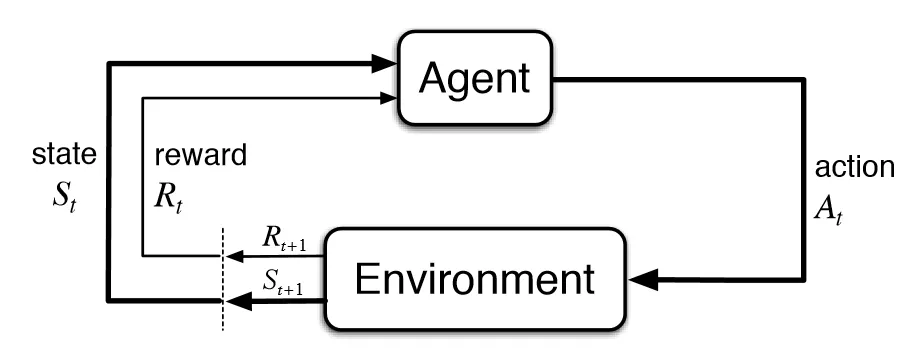
\includegraphics[width=0.6\textwidth]{Images/AgentEnvironment.png}
\caption{Interaction between the agent and the environment in a Reinforcement Learning setting \cite{sutton_reinforcement_2018}.}
\label{Figure:AgentEnvironment}
\end{figure}

The main objective of the agent is to maximise its sum of rewards, also known as the return. The return is basically the expected gain that can be achieved starting from the state \( S_t \) as expressed by this formula \cite{sutton_reinforcement_2018}:

\begin{equation}
R_{t+1} + \gamma R_{t+2} + \gamma^2 R_{t+3} + \ldots = \sum_{k=0}^{\infty} \gamma^k R_{t+k+1}
\end{equation}

Here, \( \gamma \) represents the discount factor, indicating the degree to which future rewards are considered important relative to immediate ones. A policy \( \pi \) directs the agent's actions, which can be deterministic, assigning a specific action to each state, or stochastic, assigning a probability distribution over actions. Balancing between exploration, the act of trying new actions to discover their effects, and exploitation, the act of choosing actions that are known to yield high reward, is a fundamental challenge in RL. An important approach to this problem is the \(\varepsilon\)-greedy policy, which predominantly exploits the best-known action but occasionally explores random actions, thus ensuring both robustness and continual learning \cite{sutton_reinforcement_2018}.

The fundamental concept behind Reinforcement Learning lies in the Markov Decision Process (MDP) framework, defined by the tuple \( (S, A, P, R, \gamma) \). Here, \( S \) represents all possible states in the environment, \( A \) denotes the actions the agent can take, and \( P \) is the transition probability, indicating the likelihood of moving from state \( s_t \) to state \( s_{t+1} \) after taking action \( a \). \( R \) is the return received for this transition, and \( \gamma \) is the discount factor. MDPs utilise the Markov property, ensuring that the next state depends only on the current state and action, without need to consider any past states or actions, as shown in this formula \cite{sutton_reinforcement_2018}:

\begin{equation}
\label{Equation:MarkovProperty}
P(s_{t+1} | s_t, a_t, s_{t-1}, a_{t-1}, \ldots, s_0, a_0) = P(s_{t+1} | s_t, a_t)
\end{equation}

The reward function is very important as it captures the agents objectives. It offers a signal that directs the agent towards achieving the goals of a task, but it does not prescribe how to accomplish them. For example, in the trading context, rewards can mirror gains and losses, guiding the agent to adopt strategies that maximise profits \cite{sutton_reinforcement_2018}.

\subsubsection{Value Functions and Q-Functions}

The value function for a policy \( \pi \), denoted as \( V^\pi(s) \), represents the expected return when starting in state \( s \) and following policy \( \pi \) afterwards. It is formulated as follows \cite{sutton_reinforcement_2018}:

\begin{equation}
V^\pi(s) = \mathbb{E} \left[ \sum_{k=0}^{\infty} \gamma^k R_{t+k+1} \mid S_t = s, \pi \right]
\end{equation}

Here, \( \gamma \) is the discount factor, which weighs the importance of future rewards compared to immediate rewards, and \( \mathbb{E} \) denotes the expected value, reflecting the average of all possible outcomes weighted by their probabilities. The Q-function for a policy \( \pi \), denoted as \( Q^\pi(s, a) \), represents the expected return for taking an action \( a \) in state \( s \) and following policy \( \pi \) afterwards. It is formulated as follows \cite{sutton_reinforcement_2018}:

\begin{equation}
Q^\pi(s, a) = \mathbb{E} \left[ \sum_{k=0}^{\infty} \gamma^k R_{t+k+1} \mid S_t = s, A_t = a, \pi \right]
\end{equation}

The Bellman equations, named after Richard Bellman, who first formulated them, provide a recursive decomposition for the total cumulative reward an agent can expect to receive starting from a particular state or state-action pair. These equations are fundamental to dynamic programming techniques in RL, as they express the relationship between the value of the current state or state-action pairs as the expected values of subsequent states or state-action pairs. The recursive nature of the Bellman equations allows for the iterative improvement of the estimated values, essential for the convergence of RL algorithms. This is expressed as follows \cite{sutton_reinforcement_2018}:

\begin{equation}
V^\pi(s) = \sum_{a \in A} \pi(a|s) \sum_{s' \in S} P(s'|s,a) \left[ R(s,a,s') + \gamma V^\pi(s') \right]
\end{equation}

\begin{equation}
Q^\pi(s, a) = \sum_{s' \in S} P(s'|s,a) \left[ R(s,a,s') + \gamma \sum_{a' \in A} \pi(a'|s') Q^\pi(s', a') \right]
\end{equation}

\begin{equation}
\label{Equation:RelationshipValueQFunction}
V^\pi(s) = \sum_{a \in A} \pi(a|s) Q^\pi(s, a)
\end{equation}

The relationship pointed in Equation~\ref{Equation:RelationshipValueQFunction} indicates that the value of a state under policy \(\pi\) is the expected value of the Q-function over all possible actions, weighted by the policy's action probabilities. For optimal policies, we define the optimal value function \( V^*(s) \) and the optimal Q-function \( Q^*(s, a) \), which represent the maximum possible returns achievable from any state or state-action pair, respectively. Following the Bellman equation, it is possible to obtain \cite{sutton_reinforcement_2018}:

\begin{equation}
V^*(s) = \max_{a \in A} \sum_{s' \in S} P(s'|s,a) \left[ R(s,a,s') + \gamma V^*(s') \right]
\end{equation}

\begin{equation}
Q^*(s, a) = \sum_{s' \in S} P(s'|s,a) \left[ R(s,a,s') + \gamma \max_{a' \in A} Q^*(s', a') \right]
\end{equation}

\begin{equation}
V^*(s) = \max_{a \in A} Q^*(s, a)
\end{equation}

Through the iterative application of these equations, RL algorithms gradually approximate the value and Q-functions, guiding the agent towards the optimal policy that maximises the expected cumulative reward \cite{sutton_reinforcement_2018}.

\subsubsection{Methodological Variants and Learning Methods}

The field of reinforcement learning can be divided into categories based on the properties of the learning method: model-based versus model-free, on-policy versus off-policy strategies and value-based versus policy-based techniques. 

In model-based RL, algorithms create a model of the environment to simulate and predict the outcomes of actions. This allows the agent to plan by forecasting the states. This is possible when the environment is simple enough to be modelled. On the other hand, in model-free RL, algorithms directly learn a policy or value function from their interactions with the environment without explicitly modelling it. Model-free approaches are often chosen for environments where modelling is challenging or when an accurate model is not available. Within the realm of model-free RL, there are on-policy strategies, which learn about the policy that is currently used to make decisions, and off-policy strategies, which explore a different policy while aiming to learn an optimal one \cite{sutton_reinforcement_2018}.

Another important distinction lies between value-based (also designated as critic-only) and policy-based (also designated as actor-only) learning approaches. On the one hand, value-based methods, like Temporal Difference Learning (TD), Q-Learning and SARSA Learning, focus on estimating the value of states or state-action pairs. These algorithms derive policies implicitly from these values. SARSA Learning uses an on-policy strategy, while Q-Learning and TD Learning use an off-policy strategy. On the other hand, policy-based methods, such as REINFORCE Learning, directly optimise the policy itself, which is particularly useful when dealing with continuous action spaces. In particular, Actor-Critic learning combines elements of both policy-based and value-based approaches. It has a policy function (the actor) and a value function (the critic), which provides the stability and efficiency of value-based methods along with direct policy improvement. This collaboration between the actor and the critic results in improved policy updates, especially beneficial for complex environments \cite{sutton_reinforcement_2018}. Refer to Algorithm~\ref{Codes:ActorCritic} for a detailed implementation.

\input{Codes/ActorCritic}

Although the Puterman theorem guarantees a deterministic stationary optimal policy for Markov Decision Processes (MDPs), such assurances do not extend to complex, non-stationary environments like financial markets \cite{sutton_reinforcement_2018}. Forex markets, in particular, are influenced by historical data in ways that standard state representations in MDPs do not account for. Consequently, RL in these markets relies on approximated models, utilising technical indicators and feature engineering to integrate essential historical information into the state representation in order to try to approximate the Markov property. This is why algorithms like the Actor-Critic learning are of special importance, because they act as a connection between reinforcement learning and neural networks, as we will see in the next section.

\subsection{Deep Reinforcement Learning}

Deep Reinforcement Learning (DRL) merges reinforcement learning's decision-making with the pattern recognition capabilities of neural networks, making it especially powerful for handling complex, high-dimensional data in environments like the Forex market. DRL empowers trading algorithms with adaptability, positioning them to potentially revolutionise trading strategies.

\subsubsection{Fundamentals and History}

The rise of DRL as a new field within machine learning gained momentum when it became clear that neural networks could greatly enhance the capabilities of reinforcement learning agents in dealing with and understanding complex environments. The groundbreaking work of DeepMind \cite{van_hasselt_deep_2016}, which demonstrated the success of the Double Deep Q-Network (DDQN) algorithm in mastering a range of Atari 2600 games using inputs, marked a significant breakthrough for DRL. This achievement not only validated the efficacy of DRL in mastering high-dimensional state spaces but also highlighted its potential applicability to financial markets. In this context, the challenge lies not only in interpreting large amounts of data but also in extracting strategic insights that can guide real-time trading decisions. This historical advance, along with ongoing research, has sparked interest in applying DRL to Forex trading, known to be a very volatile and dynamic environment.

\subsubsection{Deep Value-Based RL Algorithms: Deep Q-Networks}

Deep learning has transformed traditional value-based reinforcement learning methods, giving rise to what is known today as deep value-based methods. These advanced algorithms employ neural networks, known for their function approximation capabilities, to manage and interpret larger state spaces. Such an approach enables agents to learn and operate effectively in environments with complex, high-dimensional sensory input, a task that conventional value-based methods could not scale too efficiently. Neural Fitted Q-Learning was one of the early techniques that laid the foundation for deep value-based learning \cite{mnih_playing_2013}. It utilises neural networks to approximate the Q-function, which represents the expected return of a given state-action pair. By fitting a neural network to the Q-values obtained from completed episodes, it significantly enhanced the agent's ability to generalise across states in large and continuous spaces. However, the field of deep value-based methods truly came into prominence with the introduction of the Deep Q-Network (DQN) algorithm \cite{mnih_human-level_2015}. DQN integrated key innovations such as a separate target network for stabilising the learning targets and an experience replay mechanism to break the temporal correlations within training batches. This approach allowed DQN to effectively learn control policies directly from high-dimensional inputs, a significant jump forward in the application of RL. Following DQN, improvements have been made such as the Double Deep Q-Network (DDQN) to address limitations in the DQN architecture \cite{van_hasselt_deep_2016}. DDQN mitigates the overestimation bias of the action values by decoupling the action selection from the action evaluation. This is achieved by employing two networks: a primary network for action selection and a target network for evaluation, enhancing the stability and accuracy of the value estimation process. Although deep value-based methods are foundational and revolutionary, they will not be the focus of this research.

\subsubsection{Deep Policy-Based RL Algorithms: Deep Policy Gradients}

Deep policy-based RL algorithms excel in environments with continuous action spaces. Unlike value-based methods that assign a value to each potential action, policy-based approaches directly optimise the policy to maximise expected returns. This quality is invaluable in the domain of Forex trading, characterised by a vast and continuous action space that demands both precision and adaptability. Among these approaches, the Deep Deterministic Policy Gradient (DDPG) algorithm stands out as a model-free off-policy actor-critic algorithm specifically designed for continuous action spaces \cite{lillicrap_continuous_2015}. By combining the direct policy optimisation of policy-based methods with the evaluation power of value-based approaches, DDPG achieves a stable and robust learning process. The algorithm consists of an actor component for selecting actions and a critic component that evaluates the actions by estimating their Q-values. In Algorithm~\ref{Codes:DeepDeterministicPolicyGradient} we can observe how DDPG uses neural networks to approximate both the actor and critic functions. This enables handling complex input dimensions commonly encountered in Forex markets. The utilisation of a replay buffer for experience storage and the strategic sampling of mini-batches are key features that enhance learning stability by mitigating the correlation between sequential data points. Furthermore, DDPG incorporates target networks, which are gradually updated versions of the actor and critic, to solidify the learning targets and encourages gradual improvement.

\input{Codes/DeepDeterministicPolicyGradient}

Although we cannot guarantee the convergence of the DDPG due to the partially observable nature of the Forex markets, its design for continuous policy adaptation presents a good approach to developing sophisticated trading strategies. The adaptability of DDPG to the evolving conditions of financial markets and its ability to identify complex patterns highlight its potential in algorithmic trading.